\def\QRCODE{TB_image_TUT.IMG.image_registration_matlabqrcode.png}
\def\QRPAGE{http://www.iptutorials.science/tree/master/TB_image/TUT.IMG.image_registration/matlab}
\mcorrectionsection{Matlab correction}

\subsection{Transformation estimation based on corresponding points}
\subsubsection{Image visualization}
The following code is used to display the images (see Fig.\ref{fig:registration:matlab:initial}).

\begin{matlab}
A = double(imread('Brain1.bmp'));
B = double(imread('Brain2.bmp'));

figure
subplot(131);viewImage(A);title('moving image');
subplot(132);viewImage(B);title('source image')
subplot(133),imshowpair(A,B);title('superimposition');
\end{matlab}

\begin{figure}[htbp]
\centering
 \subfloat[Moving image.]{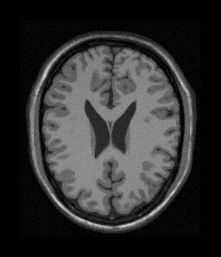
\includegraphics[width=.3\linewidth]{moving.png}}\hfill
 \subfloat[Source image.]{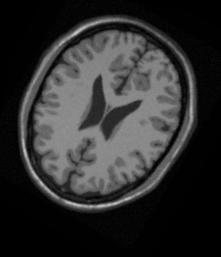
\includegraphics[width=.3\linewidth]{source.png}}\hfill
 \subfloat[Superimposition.]{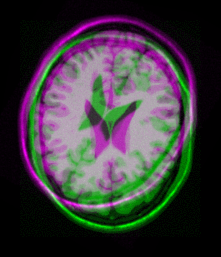
\includegraphics[width=.3\linewidth]{imageFusionReg.png}}
 \caption{Initial images.}
 \label{fig:registration:matlab:initial}
\end{figure}

If you want to save the fusion of both images, you can extract a frame, convert it into an image and save it:
\begin{matlab}
figure; imshowpair(Atrans,B);
frame = getframe();
imageFusion = frame2im(frame);
imwrite(imageFusion,'imageFusionReg.png');
close;
\end{matlab}


\subsubsection{Manual selection of corresponding points}
You just have to use the Matlab function \minline{cpselect}:
\begin{matlab}
[A_points, B_points] = cpselect(A/255,B/255);
\end{matlab}

\subsubsection{Transformation estimation}
The rigid transformation is estimated from the corresponding points by the following function (take care of the confusion between $x$ and $y$ coordinates, which is handled by \minline{fliplr} or \minline{flipud}):
\begin{matlab}
function [R, t] = rigid_registration(data1, data2)
% Rigid transformation estimation between n pairs of points
% This method finds a rotation R and a translation t
% data1 : array of size nx2
% data2 : array of size nx2

% Convert pixels coordinates into x,y coordinates
data1_inv = fliplr(data1);
data2_inv = fliplr(data2);

% computes barycenters, and recenters the points
m1 = mean(data1_inv);
m2 = mean(data2_inv);
data1_inv_shifted = data1_inv-m1;
data2_inv_shifted = data2_inv-m2;

% Evaluates SVD
K = data2_inv_shifted'*data1_inv_shifted;
[U,~,V] = svd(K);

% Computes Rotation
S = eye(2);
S(2,2) = det(U)*det(V);
R = U*S*V';

% Computes Translation
t = flipud( m2' - R*m1');
\end{matlab}

Then, you can apply this function to the manually selected points:
\begin{matlab}
%% Transformation estimation
% If coming from the previous cpselect method, the points will give an
% almost perfect transformation.
[R, t] = rigid_registration(A_points, B_points);

% if you want to evaluate the angle of rotation:
% angle_rotation = acos(R(1,1))*180/pi*sign(R(1,2))
xform = [R,[0;0];t',1];
tform_rigid = affine2d(xform);

% Matlab solution to evaluate the transformation. Notice that this is not
% exactly the same transformation, as the previous one is rigid, and this
% one allows a scaling factor.
%tform_rigid=fitgeotrans(A_points,B_points,'nonreflectivesimilarity');

% Transformation
[Atrans, Rtrans] = imwarp(A, imref2d(size(A)), tform_rigid);

% Transform of the control points
A_points_trans = R * flipud(A_points') + flipud(t);
\end{matlab}

\begin{figure}[htbp]
\centering
 \subfloat[Without registration.]{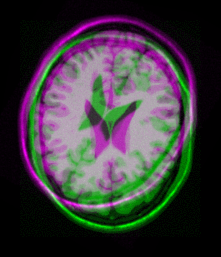
\includegraphics[width=.4\linewidth]{imageFusionReg.png}}\hfill
 \subfloat[With registration.]{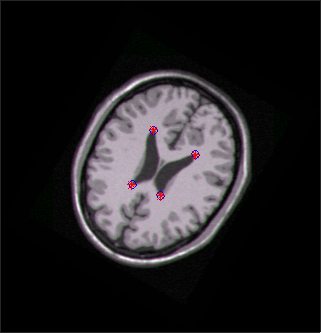
\includegraphics[width=.4\linewidth]{imageFusionManual.png}}
 
 \caption{Result of the registration for the manually selected control points.}
 \label{fig:registration:matlab:reg}
\end{figure}

The result is good, because the manual selection of the points is almost perfect.

\subsection{ICP registration}

\subsubsection{Random permutation of points}
The following code randomly shuffles the points of the first vector. The result is of course a wrongly registered image, see Fig.\ref{fig:registration:matlab:random}.
\begin{matlab}
p = randperm(length(A_points));
A_points = A_points(p,:);
\end{matlab}

\begin{figure}[htbp]
\centering
 \subfloat[Matching pairs of points.]{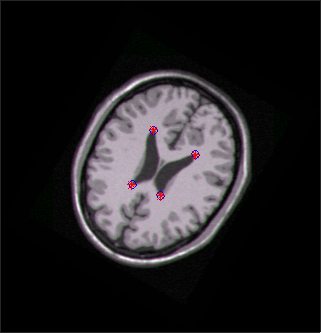
\includegraphics[width=.4\linewidth]{imageFusionManual.png}}\hfill
 \subfloat[Permulation of the points.]{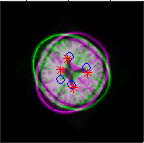
\includegraphics[width=.4\linewidth]{imageFusionRandomManual.png}}
 
 \caption{Result of the registration for when the control points are not found in the same order.}
 \label{fig:registration:matlab:random}
\end{figure}


\subsubsection{ICP}
The previous operations simulates a general non-manual selection of the control points: there is not reason to finding the points by matching pairs. Thus, a reordering is necessary. This propositions implies that the number of points is exactly the same in order to perform the registration process, and that these are matching points (every point has a matching point in the other image). The ICP method (see code for \minline{icp_transform}) reorders the points via a nearest neighbor rule.

\begin{matlab}
function tform = icp_transform(dataA, dataB)
% Find a transform between A and B points
% with an ICP (Iterative Closest Point) method.
% dataA and dataB are of size nx2, with the same number of points n 
% returns a tform affine2d object

data2A = dataA;
data2B = zeros(size(data2A));
tform=affine2d(eye(3));

nb_loops=10;
data_loop = cell(nb_loops,1);
data_loop{1} = data2A;

for loop =2: nb_loops
    % search for closest points and reorganise array of points accordingly
    [corr,~] = dsearchn(dataB, data2A);
    for j = 1:length(corr)
        data2B(j,:) = dataB(corr(j),:);
    end
    
    % find rigid registration with reordered points
    [R_loop, t_loop] = rigid_registration(data2A, data2B);
    tform_loop = affine2d([R_loop,[0;0];t_loop',1]);
    
    [X,Y]=tform_loop.transformPointsForward(data2A(:,1),data2A(:,2));
    data2A=[X,Y];
    tform = affine2d(tform_loop.T * tform.T);

    data_loop{loop} = data2A;
end
\end{matlab}

This function is then applied to the manually selected points, in random order.
\begin{matlab}
%% ICP-based image registration
% uses iterative control points algorithm, with reorganisation of points
% case with manual selection of points
% remember that A_points have been shuffled randomly
tform = icp_transform(A_points, B_points);

[Atrans, Rtrans] = imwarp(A, imref2d(size(A)), tform);
[X,Y]=tform.transformPointsForward(A_points(:,1),A_points(:,2));
A_points_trans = [Y, X]';
\end{matlab}


\begin{figure}[htbp]
\centering
 \subfloat[Random shuffle of points and direct rigid transformation estimation.]{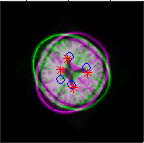
\includegraphics[width=.4\linewidth]{imageFusionRandomManual.png}}\hfill
 \subfloat[ICP registration on the same points.]{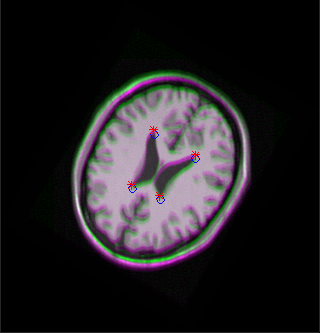
\includegraphics[width=.4\linewidth]{imageFusionICPManual.png}}
 
 \caption{Result of the registration for when the control points are not found in the same order. The ICP algorithm reorders the points and gives a good result.}
 \label{fig:registration:matlab:icp}
\end{figure}

\subsubsection{Automatic extraction of corner points}
Generally, the points are automatically detected, and thus, there is no warranty that they are found in the same order, nor that each pair of point correspond to matching points (some points --called outliers-- need to be eliminated to compute the correct transformation). In this tutorial, we do not address the problem of outliers. Please notice that with these parameters and images, by chance, the same points are detected in the correct order.

\begin{matlab}
%% Automatic extraction of corner points
% Unfortunately, this is not possible to have an interactive selection of
% the control points.
% Harris corners detection does not ensure to give the same exact points,
% in the same order.
cornersA = detectHarrisFeatures(A,'FilterSize', 7);
cornersB = detectHarrisFeatures(B,'FilterSize', 7);

nb_points = 4;
figure
subplot(121);imshow(A,[]);title('moving image');
hold on; plot(cornersA.selectStrongest(nb_points))
subplot(122);imshow(B,[]);title('source image');
hold on;
plot(cornersB.selectStrongest(nb_points));
\end{matlab}

You can pass the detected points to the rigid registration method by using:
\begin{matlab}
A_points = cornersA.selectStrongest(nb_points).Location);
\end{matlab}
The Fig.\ref{fig:registration:matlab:harris} displays the 20 strongest points for both images. Notice that there is no correspondance in these points. If you apply the previous code with these 20 points, there is a high chance that the registration will be wrong.

\begin{figure}[htbp]
\centering
 \subfloat[]{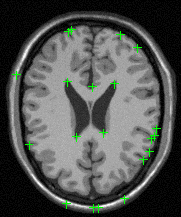
\includegraphics[width=.4\linewidth]{harris_A.png}}\hfill
 \subfloat[]{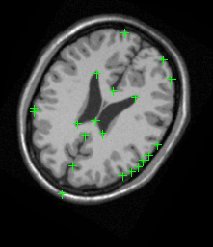
\includegraphics[width=.4\linewidth]{harris_B.png}}
 \caption{Harris corners detection. 20 points are represented.}
 \label{fig:registration:matlab:harris}
\end{figure}